\chapter{Framework}\label{ch:framework}
Im Gegensatz zu diesen etablierten Methoden basiert Predictive Maintenance auf einem völlig anderen Ansatz, der auf kontinuierlicher
Überwachung und Datenanalyse beruht. In Anlehnung an Krupitzer et al.~\cite{Krupitzer2020} werden für die Entwicklung einer Predictive
Maintenance Lösung im Kontext des SSPX1 Mautüberwachungssystems einige Rahmenbedingungen skizziert. Diese lassen sich gem.
\hyperref[fig:pdm_framework]{Abb.~\Ref*{fig:pdm_framework}} kategorisieren.

\begin{figure}[H]
    \centering
    \begin{tikzpicture}
        \node[anchor=south west,inner sep=0] (image) at (0,0) {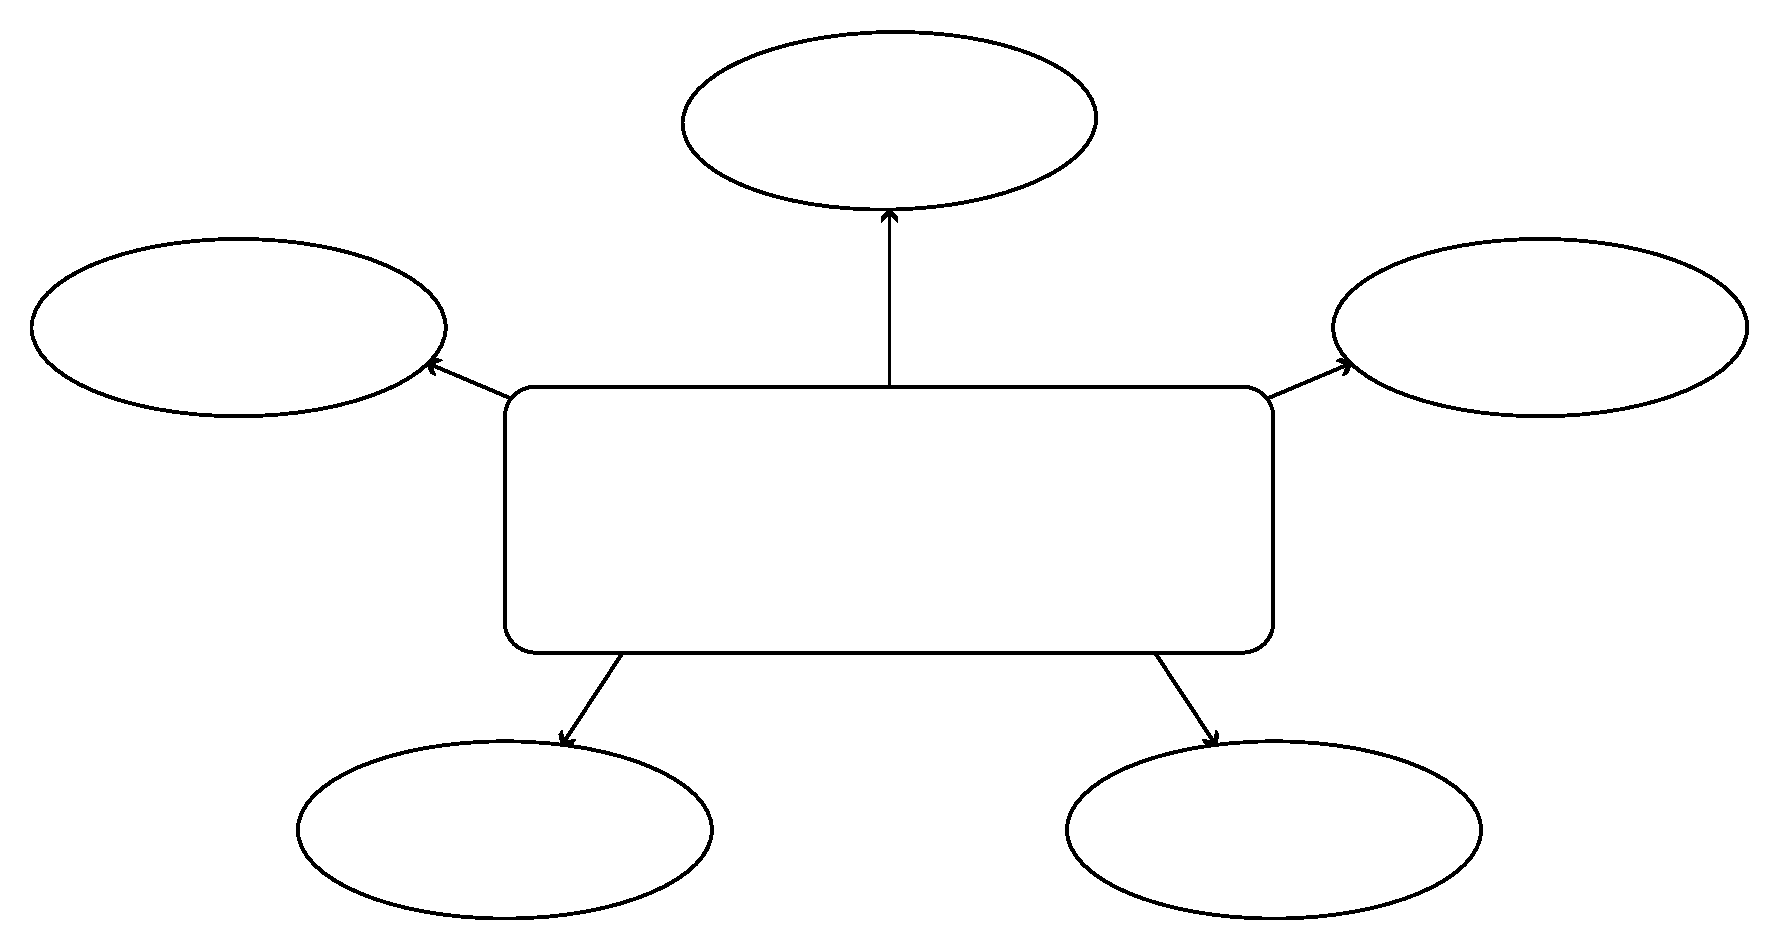
\includegraphics[width=\linewidth]{ch4_framework/abbildungen/framework.pdf}};
        % Koordinatensystem für die Grafik
        \begin{scope}[x={(image.south east)},y={(image.north west)}]
            % Textpositionen anpassen:
            \node at (0.5,0.45) {\Large\parbox{6cm}{\centering\textbf{Predictive Maintenance\\System Framework}}};
            \node at (0.13,0.65) {\large Evaluation};
            \node at (0.87,0.65) {\large \parbox{3cm}{\centering Technologische\\Grundlagen}};
            \node at (0.5,0.87) {\large Zielsetzung};
            \node at (0.28,0.13) {\large \parbox{3cm}{\centering Daten-\\verarbeitung}};
            \node at (0.72,0.13) {\large \parbox{3cm}{\centering Zustands-\\überwachung}};
            
        \end{scope}
    \end{tikzpicture}
    \caption{Framework zur Entwicklung eines Predictive Maintenance Systems}
~\label{fig:pdm_framework}
\end{figure}

\section{Technologische Grundlagen}\label{sec:technologische_grundlagen}
Die technologischen Grundlagen dieser Arbeit stützen sich auf die in der SSPX1 verbauten Sensoren, die präzise Systemdaten erfassen
und kontinuierlich überwachen. Zu den erfassten Parametern gehören unter anderem die Temperatur und Auslastung von GPU und CPU,
die Auslastung des Arbeitsspeichers sowie die Strom- und Leistungsaufnahme des Blitzermoduls.

Ein zentraler Baustein ist die Nutzung moderner IoT-Technologien in Kombination mit dem industriellen Kommunikationsstandard OPC UA.\
Dieser Standard ermöglicht einen effizienten und sicheren Zugriff auf die Sensordaten der SSPX1 und deren Übertragung an eine
Anwenderschnittstelle nach dem Client-Server-Prinzip~\cite{Babel2024}.

Da die Sensoren teilweise von unterschiedlichen Herstellern stammen und Messdaten in verschiedenen Formaten bereitstellen, sorgt OPC
UA für eine einheitliche und standardisierte Kommunikation. Die Daten werden dabei im kompakten \textit{OPC UA Binary}-Format~\cite{iec62541}
erfasst, wodurch eine performante und ressourcenschonende Datenübertragung ermöglicht wird. Anschließend werden die Daten an den OPC
UA-Server übermittelt und in der zugrundeliegenden SQL-Datenbank gespeichert. 

Durch diese Architektur wird eine herstellerübergreifende Interoperabilität gewährleistet, die OPC UA besonders für den betrachteten
Anwendungsfall geeignet macht. Die hohe Skalierbarkeit und Erweiterbarkeit des Standards ermöglicht zudem die einfache Integration
weiterer Sensoren und Systeme, wodurch zukünftige Erweiterungen ohne grundlegende Anpassungen der bestehenden Infrastruktur möglich
sind.

Ein weiterer Vorteil der Nutzung von OPC UA liegt in der serviceorientierten Architektur, die eine flexible Kommunikation
zwischen Client und Server ermöglicht. Der Client fungiert hierbei als Kommunikationsbrücke, die Anfragen und Antworten zwischen
der Anwenderschnittstelle und dem Server verwaltet. Die OPC UA-Kommunikations-Stacks unterstützen dabei die Datenverarbeitung und
gewährleisten eine robuste Übertragung, indem sie eng mit dem Speicher- und Dateisystem des Servers zusammenarbeiten. Zu den
wesentlichen Ereignissen der Client-Server-Kommunikation gehören~\cite{Babel2024,iec62541,Mao2024}:
\begin{itemize}
    \item \textbf{Message Requests:} Anfragen des Clients zur Datenabfrage oder -übertragung
    \item \textbf{Message Responses:} Antworten des Servers auf die Anfragen des Clients
    \item \textbf{Order Requests:} Aufrufe zur Ausführung bestimmter Serveraktionen
    \item \textbf{Notifications:} Benachrichtigungen über Änderungen oder Ereignisse im System
\end{itemize}

Darüber hinaus kann der OPC UA-Server als Bindeglied zwischen mehreren physischen Geräten oder auch als Cloud-Service fungieren,
was die Skalierbarkeit weiter erhöht und die Nutzung in verteilten Systemen erlaubt. Die Kombination aus präzisen Sensordaten,
standardisierter Kommunikation und einer skalierbaren Architektur bildet die technologische Grundlage für die Analyse und Umsetzung
von Predictive Maintenance im Rahmen dieser Arbeit.

\section{Zustandsüberwachung}\label{sec:zustandsueberwachung}
Ein wesentlicher Grund für ineffiziente Wartungsmaßnahmen liegt im unzureichenden Zugang zu Daten, die frühe Hinweise auf
potenzielle Schäden oder Ausfälle liefern könnten~\cite{Mobley2002}. Predictive Maintenance basiert auf der Voraussetzung, dass
Daten über den Zustand des betreffenden Systems oder der betreffenden Komponente zuverlässig verfügbar sind. Die Bereitstellung der
Daten erfolgt wie oben beschrieben mithilfe von OPC UA und die Zustandsüberwachung sensorbasiert.

Zu Beginn der Arbeit und in der Entwicklungsphase wird die Zustandsüberwachung einen inspektionsbasierten Ansatz verfolgen. Das
bedeutet, dass nach willkürlichen Intervallen immer auf die vom OPC UA Server zur Verfügung gestellten Daten zugegriffen wird und
diese Datensätze dann analysiert und weiterverarbeitet werden. Die Wahl dieser Methode basiert auf der geringeren Komplexität der
Implementierung in frühen Entwicklungsphasen und hat zur Folge, dass ein konsistenter Datensatz einen besseren Vergleich und
Feinabstimmung von Parametern der Analysetools ermöglicht.

Online Predictive Maintenance erweitert diesen Ansatz, indem sie eine kontinuierliche Überwachung des Systemzustands in Echtzeit
ermöglicht. Dabei werden Daten oder andere relevante Parameter in regelmäßigen Abständen automatisch erfasst. Nicht alle erfassten
Daten werden analysiert; vielmehr wird gezielt ausgewählt, welche Informationen für die Analyse und die Ableitung von Wartungsmaßnahmen
notwendig sind~\cite{Lindstroem2017}.

Die automatisierte Datenweiterverarbeitung als Teil der Online Predictive Maintenance erfolgt zu einem späteren Zeitpunkt und wird zu
Beginn noch nicht verfolgt, kann aber als schlussendliches Ziel gesetzt werden. So kann das in dieser Arbeit entwickelte System im
laufenden Betrieb optimal und effizient genutzt werden.

\newpage
\section{Datenverarbeitung}
Durch die kontinuierliche Aggregation von Messdaten der SSPX1 entstehen sehr große, hochdimensionale Datensätze. Jeder Datenpunkt in
der Zeitserie $S$ ist mehrdimensional. Formell lässt sich eine Zeitserie $S$ der Länge $n$ und Dimensionalität $d$ wie in
\hyperref[eq:timeseries_matrix_sum]{Gl. \Ref*{eq:timeseries_matrix_sum}a} definieren. $x_{i}^{j}$ ist der $i$-te Skalar der $j$-ten
Dimension einer Serie $S$. Für die Dimension $j={0,\dots,d}$ der Zeitserie $S$ entspricht jede Dimension einem Messwert im Datensatz. Da es
sich um eine Zeitserie handelt, entsprechen die Indizes $i={0, \dots, n}$ den Zeitstempeln der aufgenommenen Messwerte~\cite{Wenig2024}.

\begin{equation}
    \setcounter{equation}{0}
        \begin{subequations}
        \renewcommand{\arraystretch}{1.5}
        \begin{aligned}
            S &=
            \begin{bmatrix} 
                x_{0}^{0} & \cdots & x_{0}^{d} \\
                \vdots & \ddots & \vdots \\
                x_{n}^{0} & \cdots & x_{n}^{d} 
            \end{bmatrix} 
            && \text{(a)} \\[1.5em]
            S &= \sum_{i=0}^{n}\,\sum_{j=0}^{d}\,x_{i}^{j} \cdot E_{ij}
            && \text{(b)}
        \end{aligned}
    \end{subequations}
\label{eq:timeseries_matrix_sum}
\end{equation}


Alternativ kann die Zeitserie $S$ wie \hyperref[eq:timeseries_matrix_sum]{Gl. \Ref*{eq:timeseries_matrix_sum}b} in auch als Linearkombination
von Standardmatrizen geschrieben werden~\cite[S.~8]{Voigt2012}. Die elementweise Darstellung beschreibt die Matrix $S$ als Summe von
gewichteten Standardmatrizen $E_{ij}$, wobei jede Standardmatrix $E_{ij}$ genau an der Position $(i,j)$ den Wert 1 hat und sonst 0 ist.